\documentclass[../EngineeringJournal_CDavis.tex]{subfiles}

\begin{document}

%%%%%%%%%%%%%%%%%%%%%%%%%%%%%%%%%%%%%%%%%%%%%%%%%%%%%
%%%%%%%%%%%%%%%%%%%%%%%%%%%%%%%%%%%%%%%%%%%%%%%%%%%%%

\chapter[Router on a Stick]{Router\linebreak[1] On a Stick \hspace*{\fill March
8, 2020}}
\noindent\textbf{{Packet Tracer Lab 15} \hspace*{\fill}{\textbf{CIT 167}}}\linebreak[1]
{{Spring 2020} \hspace*{\fill}{Chaz Davis}}                             
%===================================
%===================================


\hspace{0.2cm}
\begin{tcolorbox}[width=6.3in]
\scriptsize 
sticks
  \begin{outline}
    \1 N shit
  \end{outline}
\end{tcolorbox}
\hspace{0.2cm}
\normalsize  
  
\clearpage

%===================================
\mysection{\textbf{Part 1: Configuring and verifying the Network}}

I First set up the network according to the diagram.
I then, Configured the Ip address, subnet masks, and default gateways for the
PCs according the chart.
I then, configured the Switch and router according to the handout.

Successfully able to ping PC3 from PC1.


\begin{figure}[!hbt]\centering
\subfloat[Pinging PC3 from
PC1]{\label{success15ping}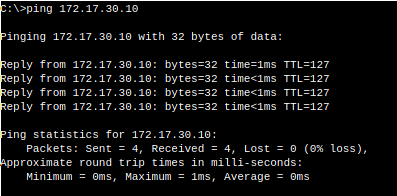
\includegraphics[width=.45\linewidth]{Figures/2020-03-08-191601_397x196_scrot.png}}\par
\subfloat[Successful Network
COnfiguration]{\label{success15net}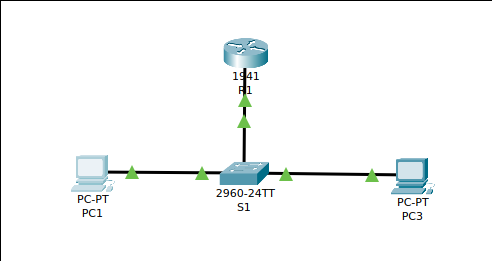
\includegraphics[width=.45\linewidth]{Figures/2020-03-08-191611_492x261_scrot.png}}\par
\caption{Successful network setup}
\label{success15}
\end{figure}








%===================================

\end{document}
